% Identification Funnel: How Each Test Narrows the Set of Explanations
% Standalone TikZ — compiled inline or via \input{}

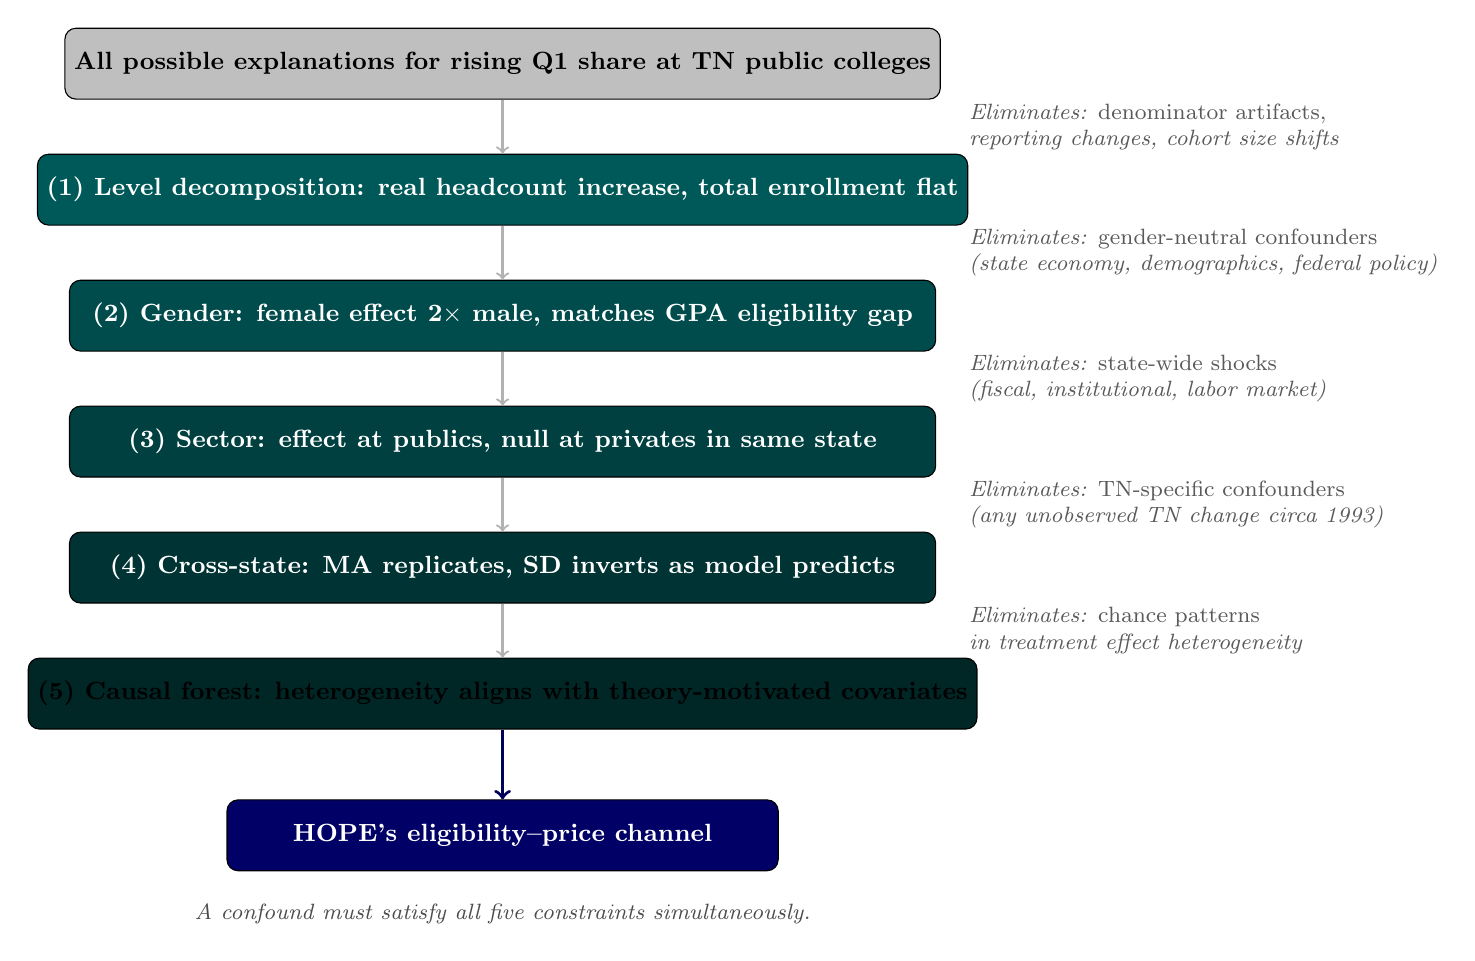
\begin{tikzpicture}[
    every node/.style={font=\small},
    block/.style={draw, rounded corners, fill=#1, minimum width=11cm,
                  minimum height=0.9cm, text=white, font=\small\bfseries,
                  align=center},
    elim/.style={font=\footnotesize, text=gray!70!black, align=left},
    arrow/.style={->, thick, gray!60},
    brace/.style={decorate, decoration={brace, amplitude=5pt, mirror}}
]

% Top: all explanations
\node[block=gray!50, text=black] (top) at (0, 0)
    {All possible explanations for rising Q1 share at TN public colleges};

% Filter 1
\node[block=teal!70!black] (f1) at (0, -1.6)
    {(1) Level decomposition: real headcount increase, total enrollment flat};
\node[elim, right] at (5.8, -0.8) {\textit{Eliminates:} denominator artifacts,\\
    \textit{reporting changes, cohort size shifts}};
\draw[arrow] (top) -- (f1);

% Filter 2
\node[block=teal!60!black] (f2) at (0, -3.2)
    {(2) Gender: female effect 2$\times$ male, matches GPA eligibility gap};
\node[elim, right] at (5.8, -2.4) {\textit{Eliminates:} gender-neutral confounders\\
    \textit{(state economy, demographics, federal policy)}};
\draw[arrow] (f1) -- (f2);

% Filter 3
\node[block=teal!50!black] (f3) at (0, -4.8)
    {(3) Sector: effect at publics, null at privates in same state};
\node[elim, right] at (5.8, -4.0) {\textit{Eliminates:} state-wide shocks\\
    \textit{(fiscal, institutional, labor market)}};
\draw[arrow] (f2) -- (f3);

% Filter 4
\node[block=teal!40!black] (f4) at (0, -6.4)
    {(4) Cross-state: MA replicates, SD inverts as model predicts};
\node[elim, right] at (5.8, -5.6) {\textit{Eliminates:} TN-specific confounders\\
    \textit{(any unobserved TN change circa 1993)}};
\draw[arrow] (f3) -- (f4);

% Filter 5
\node[block=teal!30!black, text=black] (f5) at (0, -8.0)
    {(5) Causal forest: heterogeneity aligns with theory-motivated covariates};
\node[elim, right] at (5.8, -7.2) {\textit{Eliminates:} chance patterns\\
    \textit{in treatment effect heterogeneity}};
\draw[arrow] (f4) -- (f5);

% Bottom: surviving explanation
\node[block=blue!50!black!80!black, minimum width=7cm] (bottom) at (0, -9.8)
    {HOPE's eligibility--price channel};
\draw[arrow, very thick, blue!50!black!70!black] (f5) -- (bottom);

% Challenge
\node[font=\footnotesize\itshape, text=gray!60!black, align=center] at (0, -10.8)
    {A confound must satisfy all five constraints simultaneously.};

\end{tikzpicture}
